\documentclass{scrartcl}
\usepackage[utf8]{inputenc}
\usepackage{hyperref}
\usepackage{url}
\usepackage{natbib}
\usepackage{graphicx}
\usepackage{cleveref} % this must be the last package to be loaded

\newcommand{\emailaddr}[1]{\href{mailto:#1}{\texttt{#1}}}

\title{\LARGE
    Chameleon Table\\
    A Distributed Multiplayer Card Game
}
\subtitle{Final Report for the Distributed Systems Course [2025/2026]}

% Consider watching:
% https://www.youtube.com/watch?v=ihxSUsJB_14
% https://www.youtube.com/watch?v=XTFWaV55uDo

\author{
    Andrea La Rosa \\ \emailaddr{andrea.larosa2@studio.unibo.it}
}

\date{\today}

\begin{document}

\maketitle

\begin{abstract}
Chameleon Table is a distributed multiplayer card game inspired by Coloretto,
developed as a final project for the Distributed Systems course. 
The application allows between 2 and 5 players to join a shared 
game room from different devices and play in turns, with one active
game per authenticated user. The system follows a client-server architecture:
a central FastAPI server manages game logic and state, while clients interact
through a React single-page application running in the browser.
Real-time updates are pushed to all connected clients via WebSocket,
ensuring that every player sees the current state of the game without polling.
Game state is persisted in a PostgreSQL database, so that active games
survive server restarts and players can reconnect within a grace period.
The full system is containerised with Docker and starts with a single command.
Key distributed systems challenges addressed include crash recovery,
real-time state synchronisation across multiple clients,
and safe concurrent access to shared game state.
\end{abstract}

\section*{Disclaimer}

During the preparation of this work, the author used Claude (Anthropic) to assist
with drafting and translating sections of this report, debugging backend code,
and resolving testing environment issues on Windows.

After using this tool, the author reviewed and edited the content as needed
and takes full responsibility for the content of the final report.

\section{Concept}\label{concept}

Chameleon Table is a web application inspired by the card game Coloretto,
accessible from any desktop browser without installation.
The backend exposes a REST API and a WebSocket endpoint;
the frontend is a React single-page application.

\subsection*{Use cases}

An unregistered user can sign up to the service by providing a username,
email address, and password.

A registered user can log in to the service.

An authenticated user can create a new match, choosing the maximum number of players.
The match is identified by a unique room code generated by the server.

An authenticated user can join a match that has not yet started by entering the room code,
becoming a player.

An authenticated user can observe an ongoing match without participating,
becoming an observer. The maximum number of observers per match is four.

The user who created the match can cancel it before it starts.

A player can leave an ongoing match.
If too many players leave, the match is aborted.

An observer can leave an ongoing match.

Users interact with the system through a desktop browser, in sessions lasting
the duration of a match. Turns follow each other in relatively quick succession
--- a player is expected to act within two minutes of their turn.

\subsection*{Data}

The system stores two categories of data.
User data (username, email, hashed password) is persisted in PostgreSQL.
Game state (deck, rows, players, scores) is kept in Redis during an active match
and persisted to PostgreSQL for crash recovery.

\subsection*{Roles}

There are three roles in the system:
\begin{itemize}
  \item \textbf{Guest} --- an unauthenticated user, who can only access the login and registration page.
  \item \textbf{Player} --- an authenticated user who creates or joins a match and participates actively.
  \item \textbf{Observer} --- an authenticated user who watches an ongoing match without participating.
\end{itemize}

\subsection*{Why is distribution needed?}

Distribution is needed for several reasons.
The primary one is \emph{resource sharing}: multiple players need to interact
with the same shared game state from different devices and locations simultaneously.
\emph{Fault tolerance} is also a concern: the system must survive server restarts
without losing active matches, addressed through persistence on PostgreSQL
and a reconnection grace period of two minutes.
\emph{Liveness} is guaranteed by an inactivity timer that automatically disconnects
players who do not act within two minutes of their turn, preventing matches from stalling.
Finally, the architecture is designed to allow future \emph{horizontal scaling}
via Redis pub/sub, enabling multiple backend instances to share game state.

\section{Requirements Elicitation and Analysis}\label{requirements}

\subsection{Functional Requirements}

\begin{description}
  \item[F1] The system shall allow a user to register by providing a username, email address, and password.

  \textit{Acceptance criterion: an unregistered user can create an account and subsequently log in.}

  \item[F2] The system shall allow a registered user to log in.

  \textit{Acceptance criterion: a user with valid credentials receives an access token.}

  \item[F3] An authenticated user shall be able to create a new match, specifying a maximum number of players (between 2 and 5).

  \textit{Acceptance criterion: a match is created with a unique room code, and the creator is listed as the first player.}

  \item[F4] An authenticated user shall be able to join a match that has not yet started by entering the room code.

  \textit{Acceptance criterion: the player appears in the match player list, and all other players already in the match receive the updated state.}

  \item[F5] The player who created the match shall be able to start it once the number of players specified at creation has been reached.

  \textit{Acceptance criterion: the match transitions to the PLAYING phase and all players in the match receive the updated state.}

  \item[F6] The player who created the match shall be able to cancel it before it starts.

  \textit{Acceptance criterion: the match transitions to the ABORTED phase and all waiting participants are notified.}

  \item[F7] During their turn, a player shall be able to draw a card from the deck.

  \textit{Acceptance criterion: the card is removed from the deck and assigned as the pending card.}

  \item[F8] After drawing a card, a player shall be able to place it on an available row.

  \textit{Acceptance criterion: the card appears on the chosen row and the turn passes to the next player.}

  \item[F9] A player shall be able to take all the cards assigned to a row.

  \textit{Acceptance criterion: the cards of the row are assigned to the player and the row is marked as taken.}

  \item[F10] A player shall be able to leave an ongoing match.

  \textit{Acceptance criterion: the player is set to inactive status.}

  \item[F11] A match shall be automatically aborted if at least two players leave, or if only one player remains active.

  \textit{Acceptance criterion: the match transitions to the ABORTED phase and all connected clients are notified.}

\item[F12] An authenticated user shall be able to observe an ongoing match without participating in it.

  \textit{Acceptance criterion: the observer receives real-time state updates without being able to perform any game action.}

  \item[F13] An observer shall be able to leave the match they are observing.

  \textit{Acceptance criterion: the observer is removed from the observer list and no longer receives state updates.}

  \item[F14] The system shall allow a disconnected player to reconnect within a two-minute grace period.

  \textit{Acceptance criterion: a player who reconnects within the grace period resumes playing normally.}

  \item[F15] The system shall detect connected but inactive players and automatically disconnect them after two minutes of inactivity on their turn.

  \textit{Acceptance criterion: a player who does not act within two minutes is disconnected and the grace period timer starts.}

  \item[F16] Active matches shall survive a server restart.

  \textit{Acceptance criterion: after a server restart, active matches are restored and players can reconnect.}

  \item[F17] An authenticated user shall be able to view the list of available matches, including those waiting for players and those currently in progress.

  \textit{Acceptance criterion: the user can see waiting matches to join and ongoing matches to observe.}

  \item[F18] At the end of a match, all players shall be able to view the final scores.

  \textit{Acceptance criterion: once the match transitions to the FINISHED phase, the scores of all players are displayed.}

  \item[F19] The number of observers per match shall not exceed four.

  \textit{Acceptance criterion: a fifth user attempting to observe a match receives an error and is not added to the observer list.}

\end{description}

\subsection{Non-functional Requirements}

\begin{description}
  \item[NF1] Game state updates shall be transmitted in real time to all connected clients (polling excluded).

  \textit{Acceptance criterion: all connected clients receive the update within a reasonable time from the action that generated it.}

  \item[NF2] The game state shall be consistent across all connected clients.

  \textit{Acceptance criterion: all clients see the same game state at any given moment.}

  \item[NF3] The system shall guarantee match liveness; player inactivity shall not cause a match to stall.

  \textit{Acceptance criterion: no match remains blocked indefinitely due to an inactive or disconnected player.}

  \item[NF4] The system shall ensure that only authenticated users can access game features.

  \textit{Acceptance criterion: requests without a valid token are rejected by the system (error 401).}

  \item[NF5] The system shall ensure that each user can only perform actions allowed by their role.

  \textit{Acceptance criterion: an observer cannot perform game actions; a player cannot act outside their turn.}

\end{description}
\subsection{Implementation Requirements}

\begin{description}
  \item[I1] Data persistence shall be handled by PostgreSQL.

  \textit{Motivation: the need for a robust relational database for crash recovery and predisposition to future failover architectures.}

  \item[I2] The in-memory game state shall be managed via Redis.

  \textit{Motivation: the need for low latency in the most frequent operations and predisposition to future horizontal scaling via pub/sub.}

  \item[I3] The entire system shall be containerised with Docker and startable with a single command.

  \textit{Motivation: guarantees portability and reproducibility of the environment.}

  \item[I4] Real-time communication shall take place via WebSocket.

  \textit{Motivation: necessary to guarantee NF1.}

  \item[I5] The system shall expose a REST API for room management and authentication.

  \textit{Motivation: explicit requirement of the course.}

\end{description}


\subsection{Relevant Distributed System Features}
\label{ds-features}

\subsubsection*{Relevant}

\begin{description}
  \item[Fault tolerance] The system must survive server crashes, client disconnections,
  and player inactivity. Data loss of an active match is unacceptable.
  The system addresses this through crash recovery on PostgreSQL,
  a two-minute reconnection grace period,
  and an inactivity timer that automatically disconnects inactive players.

  \item[Resource sharing] Multiple clients concurrently access the same shared game state.
  Concurrent access is protected by a per-room lock (\texttt{asyncio.Lock})
  that serialises operations on the state, guaranteeing consistency.

  \item[Security] The system manages user data and requires JWT authentication
  to access game features.
  Authorisation is role-based: during a match, an observer cannot perform game actions
  and a player can only act during their own turn.

  \item[Performance and concurrency] The server manages multiple matches simultaneously.
  Update latency must be low to guarantee a good gaming experience;
  for this reason WebSocket is used instead of polling,
  and Redis serves as the fast-access layer for game state.
\end{description}

\subsubsection*{Partially relevant}

\begin{description}
  \item[Transparency] The client is unaware of the internal details of the system
  (Redis, PostgreSQL, locks). It only sees the game state updated via WebSocket.

  \item[Scalability] The system is single-instance, but the architecture is designed
  for future horizontal scaling via Redis pub/sub.

  \item[Evolvability] The architecture is designed to be extended:
  not only for scaling via Redis pub/sub,
  but also for failover via PostgreSQL and future features via JWT.
\end{description}

\subsubsection*{Not addressed}

\begin{description}
  \item[Openness and interoperability] Although standard protocols are used,
  interoperability with external systems has not been considered.

  \item[Economy] No cost evaluation has been performed.
\end{description}

\section{Design}\label{design}

This chapter explains the strategies used to meet the requirements identified in the analysis.

\subsection{Architecture}\label{architecture}

The client-server architecture is a natural choice for a digitalised board game.
Established platforms in the sector, such as Boardgame Arena and Chess.com,
adopt the same approach for reasons that apply to Chameleon Table as well.

The sole authority over the game state is the centralised server, in order to
guarantee information hiding.
The deck, the order of the cards, and information private to individual players
are never transmitted to clients, preventing a dishonest client from accessing
data outside its scope or altering the game state in its favour.
The server is also the only entity authorised to determine who can act and when,
guaranteeing the correctness of the turn order.

Crash recovery is simplified by centralisation.
Since a match can last several minutes and many matches may run simultaneously,
client-side crashes are frequent and inevitable; a peer-to-peer architecture
would require strong coordination among participants.
With a centralised server it is sufficient to maintain an up-to-date snapshot
for each match: if the server crashes, the match is restored on restart;
if a client crashes, the player can simply reconnect within the grace period.

Anomalous system states --- disconnections, prolonged inactivity, abandonments ---
are handled centrally without burdening individual clients,
which in a peer-to-peer model would be responsible for this logic.

The main drawback of this architecture is the single point of failure:
a server crash interrupts all ongoing matches.
This risk is mitigated through crash recovery on PostgreSQL,
but a multi-instance architecture with automatic failover would offer stronger guarantees.

\subsection{Infrastructure}\label{infrastructure}

The system infrastructure is composed of five components, all running as Docker
containers orchestrated by Docker Compose.

\textbf{Nginx} is the sole entry point for all incoming traffic.
It acts as the system's reverse proxy, routing requests to the appropriate
internal service based on the URL path:
\texttt{/} to the frontend,
\texttt{/api/} to the backend REST API,
and \texttt{/ws/} to the backend WebSocket endpoint.
Rate limiting is also enforced to protect the backend from overload.

\textbf{Frontend} is a React single-page application composed of static files,
not directly reachable from outside the Docker network.

\textbf{Backend} is the FastAPI application server; it manages game logic,
state, authentication, and WebSocket connections.
It is not directly reachable from outside the Docker network.

\textbf{PostgreSQL} is the relational database used for persistent storage of
user data and game state snapshots. It is only reachable internally.

\textbf{Redis} serves as an in-memory data store used as the fast-access layer
for active game state. It is only reachable internally.

All components reside on the same host and communicate over a shared internal
Docker network. Components discover each other via Docker Compose's built-in
DNS resolution: each service is reachable by its own name
(\texttt{backend}, \texttt{db}, \texttt{redis}, etc.).
Only the Nginx container exposes a port to the outside world
(port 80 in development, ports 80 and 443 in production).

In the development environment, all containers run on a single Windows machine
with Docker Desktop, and the browser runs on the same machine.
In the production environment, all containers run on a single virtual machine
on Google Cloud Platform; the browser runs on the users' devices,
which are geographically distributed.
A DuckDNS domain name points to the public IP address of the VM,
and Let's Encrypt provides the TLS certificate for HTTPS.

\begin{figure}
    \centering
    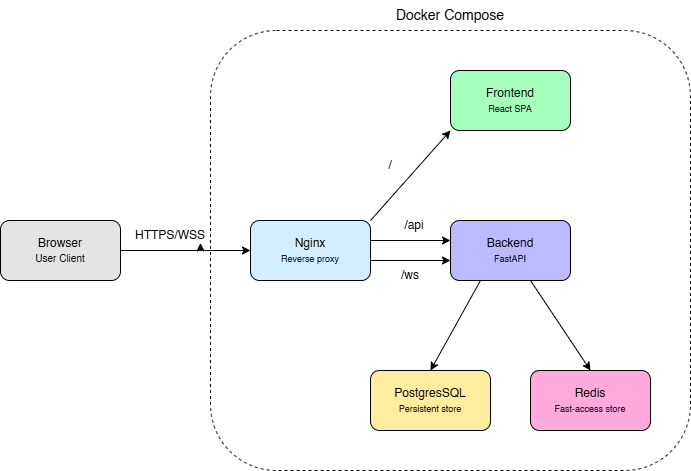
\includegraphics[width=0.8\textwidth]{figures/infrastructure.png}
    \caption{Infrastructure component diagram}
    \label{fig:infrastructure}
\end{figure}
\subsection{Modelling}\label{modelling}

\subsubsection*{Domain entities}

The main domain entities are:

\begin{description}
  \item[User] A registered user, identified by username, email and password.
  They can take the role of Player or Observer during a match.

  \item[Match (GameState)] A match, identified by a unique room code.
  It is the central entity of the system and contains all the state
  necessary for the match to proceed.

  \item[Player] A user who actively participates in a match.
  They have a hand of cards, a set of jokers, and a status
  that can be active, inactive, or permanently left.

  \item[Observer] A user who watches an ongoing match without participating.
  They have no cards and no turns.

  \item[Card] A game card, characterised by a type
  (\texttt{color}, \texttt{joker}, \texttt{plus2}, \texttt{last\_round})
  and optionally by one of seven available colours.

  \item[Row] One of the rows on the game board.
  It contains the cards placed during the turn and can be taken by a player.
\end{description}

\subsubsection*{Mapping to infrastructural components}

The complete state of each match resides exclusively on the server.
During an active match, the state is kept in Redis to guarantee low latency;
a copy is persisted to PostgreSQL on every significant change for crash recovery.
Clients maintain no authoritative state: they receive full state snapshots
from the server via WebSocket and only display them.
This guarantees consistency --- there is a single source of truth.
Information hiding is achieved by providing each client only with the information
appropriate to its role.

User data (username, email, and hashed password) is persisted only in PostgreSQL
and never passes through Redis.

\subsubsection*{Domain events}

The main events that modify the system state are:

\begin{itemize}
  \item Match: created, started, aborted, finished
  \item Player: joined, left, disconnected, reconnected
  \item Card: drawn, placed
  \item Row taken
  \item Round ended
  \item Observer: joined, left
\end{itemize}

\subsubsection*{Messages exchanged}

Messages fall into two categories.
\emph{REST commands} are sent from the client to the server to request an action
and receive a synchronous response with the updated state.
\emph{WebSocket events} are sent by the server to all clients connected to a room
whenever the state changes.
Each message contains the full snapshot of the match state --- not just the delta ---
to simplify client-side handling and ensure that a reconnecting client
immediately receives a consistent state.
Each message includes a monotonically increasing sequence number
that allows the client to discard messages arriving out of order or as duplicates.

\subsubsection*{System state}

The global state comprises the set of registered users and the set of active matches.
For each match, the state includes:

\begin{itemize}
  \item the remaining deck of cards
  \item the rows on the board
  \item the list of players with their respective cards and jokers
  \item the current turn
  \item the match phase (\texttt{WAITING}, \texttt{PLAYING}, \texttt{FINISHED}, \texttt{ABORTED})
  \item the list of observers
  \item the card currently awaiting placement (\texttt{pending\_card})
  \item the current sequence number
\end{itemize}

The domain model is shown in \cref{fig:entity}.

\begin{figure}
    \centering
    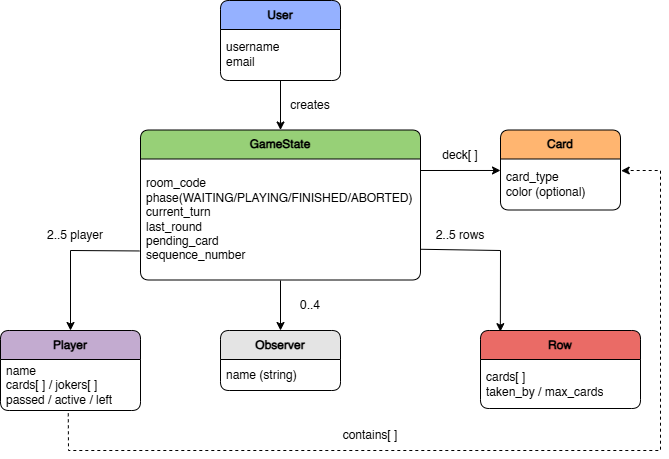
\includegraphics[width=0.85\textwidth]{figures/entity_diagram.png}
    \caption{Domain model diagram}
    \label{fig:entity}
\end{figure}
\subsection{Interaction}\label{interaction}

\subsubsection*{Interaction patterns}

The system uses two distinct interaction patterns, each suited to a different
type of communication.
Registration, login, room creation and joining, match start, and leave operations
use the synchronous \emph{request-response} pattern via REST.
The client sends an HTTP request to the server through Nginx and receives a
synchronous response containing the outcome of the operation and the updated state.
These operations modify the system state and require JWT authentication
in the request header.

Real-time game operations use the asynchronous \emph{push} pattern via WebSocket.
Each client connected to a room maintains a persistent WebSocket connection
with the server.
Whenever the state changes --- following a REST action --- the server broadcasts
the new state to all clients connected to the room.
The client does not request updates; it receives them automatically.
This guarantees that all participants always see the same game state without polling.

\subsubsection*{Concurrency}

Multiple clients may send requests to the same room simultaneously.
To guarantee state consistency, each room is protected by an exclusive lock
(\texttt{asyncio.Lock}).
The backend acquires the corresponding lock before every read or write
on a match's state.
This serialises operations on the same room, preventing race conditions.
Locks on different rooms do not block each other, guaranteeing parallelism
across distinct matches.

\subsubsection*{Messages and consistency}

Every WebSocket message includes a monotonically increasing sequence number.
The client tracks the last received sequence number and discards messages
with a lower or equal number, rejecting duplicates or out-of-order messages.
This is particularly relevant in reconnection scenarios, where delayed messages
could overwrite a more recent state.

All messages contain the full snapshot of the match state.
Compared to delta-based updates, this approach simplifies client-side handling
and eliminates the need to maintain an incremental state:
a reconnecting client immediately receives a consistent state without having
to reconstruct the history of previous events.

\subsubsection*{WebSocket --- connection and reconnection}

On connection, the backend verifies the JWT token passed as a URL parameter.
If the token is valid and the room exists, the client is added to the
connected list and immediately receives a full snapshot of the current match state.

In the event of an involuntary disconnection, the backend sets the player
as inactive and starts a two-minute grace period timer.
During this period, the other clients receive a broadcast notifying them
of the player's inactivity.
If the player reconnects within the grace period, the timer is cancelled,
the player is reactivated, and all clients receive a new broadcast.
If the timer expires without reconnection, the player is considered to have
left permanently. Under specific conditions, the match is aborted.

\subsubsection*{Nginx}

Nginx is not a passive proxy.
For REST requests, it enforces rate limiting to protect the backend from overload.
For WebSocket connections, it handles the HTTP $\rightarrow$ WebSocket protocol
upgrade via the \texttt{Upgrade} and \texttt{Connection} headers,
and keeps the connection open without timeout for the entire duration of the match.
The client always communicates exclusively with Nginx and is unaware of the
existence of the backend, Redis, or PostgreSQL.

The sequence diagrams in \cref{fig:seq_draw} and \cref{fig:seq_ws} illustrate
respectively the flow of a game move and the WebSocket connection/reconnection flow.

\begin{figure}
    \centering
    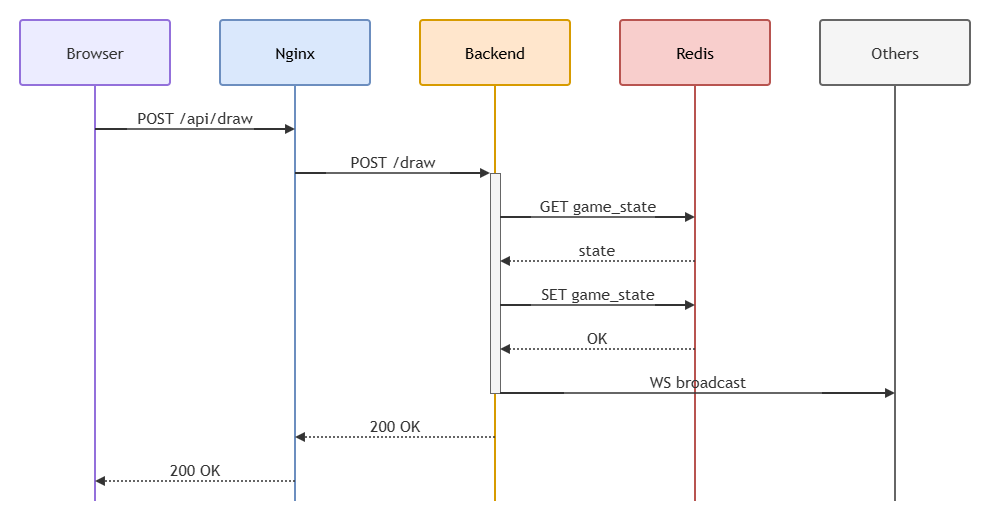
\includegraphics[width=0.85\textwidth]{figures/draw_card.png}
    \caption{Sequence diagram: draw card flow}
    \label{fig:seq_draw}
\end{figure}

\begin{figure}
    \centering
    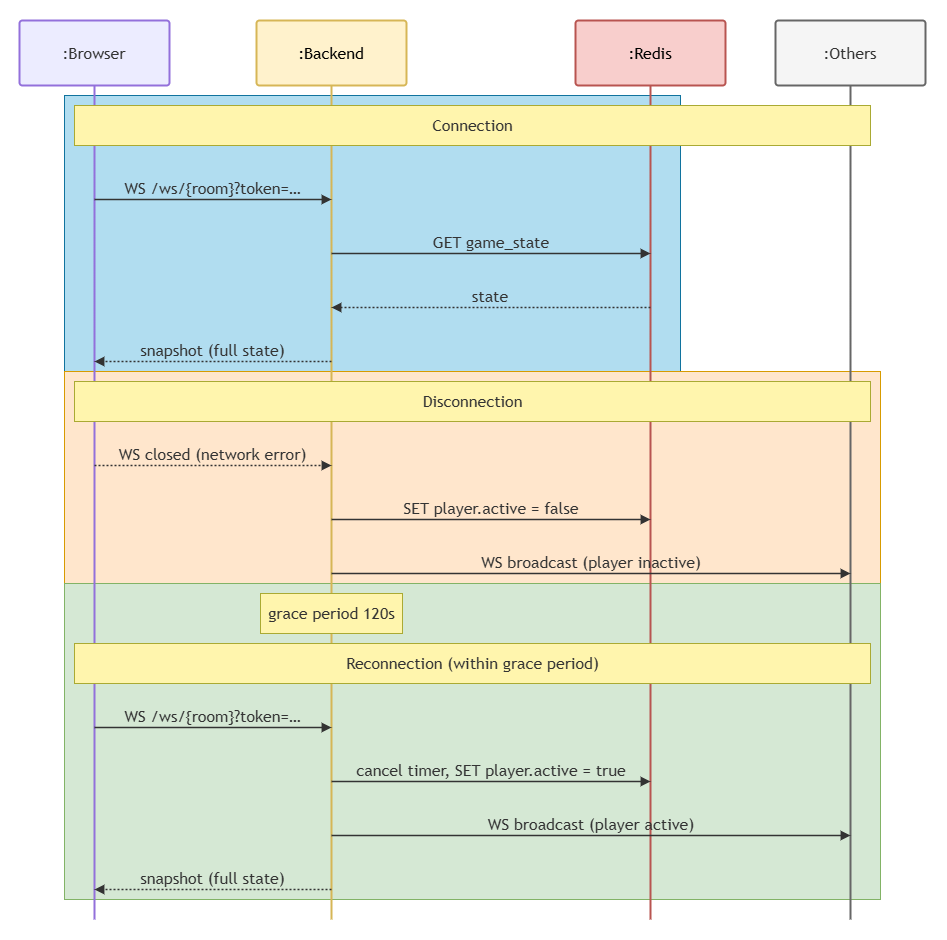
\includegraphics[width=0.85\textwidth]{figures/grace_time.png}
    \caption{Sequence diagram: WebSocket connection and reconnection}
    \label{fig:seq_ws}
\end{figure}

\subsection{Behaviour}\label{behaviour}

\subsubsection*{Stateful components}

\textbf{Redis} holds the in-memory state of all active matches.
It is the component that the backend reads and updates on every game operation.
The state is volatile --- in the event of a Redis crash the data would be lost ---
but this is prevented by PostgreSQL.

\textbf{PostgreSQL} is stateful.
It holds the persistent storage of user data and match snapshots.
It survives server crashes and enables crash recovery on restart.

\textbf{The backend} is the central and logically stateful component.
It is the sole entity responsible for updating the system state.
It handles REST requests from clients, updates the state in Redis,
persists to PostgreSQL, and notifies all clients via WebSocket broadcast.
It also manages asynchronous timers for player disconnection and inactivity.

\subsubsection*{Stateless components}

\textbf{Nginx} is completely stateless.
It only routes requests to the appropriate service based on the URL path
and handles the WebSocket upgrade.
It maintains no information about the state of matches or users.

\textbf{The frontend} is stateless from an authoritative point of view.
It locally maintains a copy of the match state received via WebSocket,
but this copy is purely for display purposes.
It makes no game decisions and does not modify the system state autonomously.

\subsubsection*{Match lifecycle}

The match itself is behaviourally interesting; it is modelled as a finite state
machine with four states:

\begin{description}
  \item[WAITING] The match has been created and players are joining.
  In this state players can be added, and the creator can start or cancel the match.

  \item[PLAYING] The match is in progress. Players take turns.
  The state transitions to \texttt{FINISHED} after the last round is completed
  following the drawing of the \texttt{last\_round} card.
  It transitions to \texttt{ABORTED} if too many players leave
  or disconnect permanently.

  \item[FINISHED] The match has ended normally.
  The final scores are available.

  \item[ABORTED] The match has been interrupted, either before it started
  due to cancellation by the creator, or during the match due to
  too many players leaving.
\end{description}

The state diagram in \cref{fig:state} illustrates the transitions between
states with their guards and triggers.

\begin{figure}
    \centering
    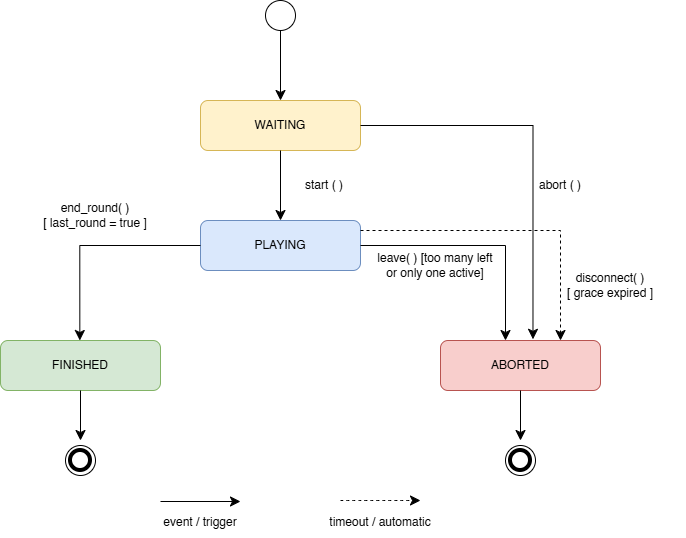
\includegraphics[width=0.85\textwidth]{figures/state_diagram.png}
    \caption{Match lifecycle state diagram}
    \label{fig:state}
\end{figure}

\subsection{Data and Consistency Issues}\label{data-and-consistency-issues}

\subsubsection*{Data}

The system manages two categories of data with different characteristics
and requirements.

User data --- username, email, and hashed password --- is persisted exclusively
in PostgreSQL in relational form.
It is written once at registration and read at every login.
It never passes through Redis.

Match state is the most critical and frequently updated data.
It is kept in Redis during the match to guarantee low latency,
and persisted to PostgreSQL on every significant change
(match start, card drawn, row taken, round ended, player left)
for crash recovery.
PostgreSQL stores the snapshots in serialised form.

\subsubsection*{Consistency}

The main risk of inconsistency is concurrent access to a room's state
from multiple simultaneous REST requests.
This is resolved through an exclusive per-room lock (\texttt{asyncio.Lock}).
Every operation that reads or modifies the state acquires the lock before
proceeding and releases it upon completion.
This guarantees that operations on the same room are serialised.

The WebSocket broadcast always occurs within the lock, after the state
has been updated in Redis.
This guarantees that all clients always receive a consistent and up-to-date state.

\subsubsection*{Shared data between components}

The backend is the only component that reads from and writes to Redis.
PostgreSQL is used only for persistence and recovery, not for real-time operations.
There is no direct state sharing between multiple backend instances,
as the system is single-instance.

The architecture is designed for future horizontal scaling:
by introducing Redis pub/sub, multiple backend instances could share match state,
replacing the in-process lock with a distributed Redis lock.

\subsection{Fault-Tolerance}\label{fault-tolerance}

\subsubsection*{Data replication and persistence}

Match state is managed on two levels to balance performance and safety.

\begin{description}
  \item[In-memory (Redis)] Used during gameplay to minimise latency.
  \item[Persistent (PostgreSQL)] On every relevant event or state change,
  the state is saved to the database as a snapshot.
\end{description}

The synchronisation between the two systems is not transactional and is therefore
not intended to guarantee high availability in real time.
PostgreSQL acts as a safety anchor for crash recovery: in the event of a server
crash, the system restarts from here.

\subsubsection*{Server crash recovery}

On startup, the backend queries PostgreSQL to retrieve all matches that were
in the \texttt{PLAYING} state at the time of the crash.
To restore the session without penalising any player:

\begin{enumerate}
  \item All players in the match are temporarily set to inactive.
  \item A two-minute grace period timer is started.
  \item If clients reconnect within the timeout, they resume the match
  from where they left off; otherwise, they are considered permanently disconnected.
\end{enumerate}

\subsubsection*{Involuntary client disconnection}

If a client loses its connection (detected via WebSocket closure),
a two-minute grace period timer is started to allow reconnection.
In the meantime, the match continues normally for the other participants.

If the player reconnects within the grace period, the timer is stopped
and the player becomes active again.
If the timer expires, the player is removed from the match.
If their absence makes it impossible to continue, the match is aborted.

\subsubsection*{Inactivity handling (anti-stall)}

To prevent a user from blocking the match by not playing their turn,
an inactivity timeout of two minutes is enforced.
Once this limit is exceeded, the system forces the client's disconnection,
which then triggers the standard grace period timer described above.

\subsubsection*{Database resilience (PostgreSQL down)}

All queries to PostgreSQL are wrapped in \texttt{try/except} blocks.
If the database goes offline, the system does not crash: matches continue
to run using Redis only.
In this degraded scenario, crash recovery is not guaranteed,
and the anomaly is immediately logged at warning level on the server.

\subsection{Availability}\label{availability}

\subsubsection*{State caching}

To avoid overloading the relational database, Redis is used as a cache
for active match state.
Every game action reads and writes directly in memory,
avoiding continuous queries to PostgreSQL during the match.
The main advantage is minimal latency and reduced load on the database.

\subsubsection*{Load balancing and scalability}

The system is currently single-instance, so there is no load balancing.
Nginx acts as a reverse proxy but only forwards requests to a single backend
server without distributing the load across multiple machines.
As discussed in the Data and Consistency section, the architecture has been
designed to support future horizontal scaling via Redis pub/sub.

\subsubsection*{Network partitioning}

If the network between clients and server goes down, clients lose their
WebSocket connection.
From the backend's perspective, this situation is indistinguishable from
a normal disconnection, so the standard two-minute grace period timer is started.

If the network issue resolves within the timeout, clients reconnect
and resume without problems.
If the outage lasts more than two minutes, the players are disconnected
permanently and, depending on the conditions, the match is aborted.

In general, in the event of a network partition the system prioritises
\emph{consistency} over \emph{availability}: it is preferable to abort a match
rather than continue it with a potentially corrupted or misaligned state.

\subsection{Security}\label{security}

\subsubsection*{Authentication and session management}

Access to all game features is entirely conditional on authentication,
which is handled via JWT (JSON Web Token).
At registration, the user's password is hashed using bcrypt before being
saved to PostgreSQL; passwords are never stored in plain text under any circumstances.

When a user logs in, the server validates the credentials and returns a signed
JWT token.
Clients must then include this token in the \texttt{Authorization} header
for standard REST calls, or as a URL parameter when establishing
a WebSocket connection.

\subsubsection*{Authorisation and role logic}

The backend implements role-based access control, verifying the user's identity
on every request.
The server ensures that each action is consistent with the player's role
and the match state. Specifically:

\begin{itemize}
  \item Only active players can perform game moves
  (drawing cards, placing them, or taking rows).
  \item Lobby management (starting or cancelling the match) is reserved
  exclusively for the match creator.
  \item Observers can only watch and cannot perform any game action.
  \item A player cannot act outside their own turn under any circumstances.
\end{itemize}

All these checks are enforced server-side and cannot be bypassed
by modifying the client.

\subsubsection*{Cryptographic schemes}

For the protection of sensitive data, well-established standards are used.
Passwords are hashed with bcrypt, an adaptive hashing algorithm that provides
strong resistance against brute-force attacks.
JWT tokens are signed with HMAC-SHA256 using a secret key stored
in environment variables.
In the production environment, all traffic is encrypted over HTTPS and WSS
to prevent man-in-the-middle attacks.

\subsection{Implementation}\label{implementation}

\subsubsection*{Network protocols and communication}

Two different approaches are combined depending on the requirements.
HTTP/1.1 is used for all standard REST calls: account management
(registration, login), room creation, and game actions.
For everything that requires real-time updates, clients open and maintain
a persistent WebSocket connection, which is used to instantly receive
state changes from the backend.

\subsubsection*{Data format}

Both REST and WebSocket communication use JSON as the interchange format.
Payloads travel with JSON bodies and responses return the match state
serialised in the same way.
On the backend, Pydantic handles validation and serialisation;
on the frontend, the standard JavaScript methods
(\texttt{JSON.parse} and \texttt{JSON.stringify}) are used.

\subsubsection*{Database interaction}

Interaction with PostgreSQL goes through SQLAlchemy in asynchronous mode,
using the \texttt{asyncpg} driver.
SQLAlchemy's ORM is used to write queries in standard SQL without
burdening the codebase.
The connection to Redis is also asynchronous, managed via the \texttt{redis-py}
library.
Match state is serialised to a JSON string before being saved in Redis;
on reading, \texttt{dacite} is used to reconstruct the Python dataclasses.

\subsubsection*{Authentication and authorisation}

The JWT mechanism is handled with the \texttt{python-jose} library.
Tokens include a configurable expiry and are signed with HMAC-SHA256.
Passwords are hashed with bcrypt via \texttt{passlib}.
The \texttt{/login} endpoint validates the user and issues the token;
protection of subsequent routes is delegated to a FastAPI dependency
(\texttt{get\_current\_user}) injected directly into the protected endpoints.

For permissions, no external RBAC framework has been introduced to avoid
overcomplicating the project.
Everything is checked explicitly server-side: each endpoint manually verifies
that the user meets the requirements for that specific action
(for example, checking whether it is their turn, whether the match is
in the \texttt{PLAYING} state, or whether the user is an active player).

\subsection{Technological details}\label{technological-details}

\begin{description}
  \item[FastAPI] Chosen as the main backend framework for its strong async
  performance and native support for WebSocket and Pydantic.

  \item[React + Zustand] For the frontend user interface, using Zustand
  to manage global state in a lightweight way.

  \item[PostgreSQL \& Redis] The former for long-term persistence,
  the latter as an in-memory data store for active matches.

  \item[SQLAlchemy \& dacite] Respectively the async ORM and the tool
  for converting dictionaries into dataclasses.

  \item[Nginx \& Docker Compose] Nginx acts as a reverse proxy also handling
  WebSocket connections and rate limiting; Docker Compose orchestrates
  the containers both locally and in production.

  \item[python-jose, passlib/bcrypt \& Pydantic] For security, password
  hashing, and data validation.

  \item[pytest \& pytest-asyncio] The framework used to run asynchronous tests.
\end{description}

\section{Validation}\label{validation}

\subsection{Automatic Testing}\label{automatic-testing}

The backend was developed following a Test-Driven Development (TDD) approach.
All tests are implemented using \texttt{pytest} and \texttt{pytest-asyncio},
and can be run with a single command from the project root:

\begin{verbatim}
pytest tests/ -v
\end{verbatim}

The suite comprises 73 tests in total, structured into two macro-categories:
unit tests and integration tests.

\subsubsection*{Unit Tests}

Unit tests verify the correctness of the game logic in complete isolation,
without involving the network, the database, or Redis.
For each test, the \texttt{GameState} object is instantiated using helper
functions defined in \texttt{tests/conftest.py}, which then invoke the pure
functions in \texttt{backend/game.py}.

\begin{description}
  \item[\texttt{test\_deck.py}] Verifies deck initialisation and the initial
  game state. \textit{Requirements covered: F3, F5.}

  \item[\texttt{test\_turns.py}] Verifies the correct management and
  alternation of turns. \textit{Requirements covered: F7, F8, F15.}

  \item[\texttt{test\_round.py}] Verifies round management and the related
  state transitions. \textit{Requirements covered: F9, F18.}

  \item[\texttt{test\_score.py}] Verifies the score calculation algorithm.
  \textit{Requirements covered: F18.}

  \item[\texttt{test\_observers.py}] Verifies the management and tracking
  of observers in a match. \textit{Requirements covered: F12, F13, F19.}

  \item[\texttt{test\_two\_players.py}] Verifies the application of the
  special rules for two-player matches. \textit{Requirements covered: F3.}
\end{description}

\subsubsection*{Integration Tests}

Integration tests verify the interaction between the different software
components through the full HTTP stack, including the authentication module,
routing, game logic, and state persistence on Redis and PostgreSQL.

Available in \texttt{tests/api/test\_integration.py}, these tests use
\texttt{httpx.AsyncClient} with \texttt{ASGITransport} to make direct calls
to the FastAPI application, simulating client-server interaction without
the overhead of a real network connection.

The test environment is isolated by setting the \texttt{TESTING=1} environment
variable, which forces the backend to connect to a dedicated test database.
PostgreSQL and Redis run inside Docker containers, exposing the necessary
ports to the local environment.

The integration suite comprises 25 tests, organised by logical domain.

\paragraph{Authentication}
\begin{description}
  \item[\texttt{test\_register}] Verifies that a new user can register and
  that the response contains the correct username (F1).

  \item[\texttt{test\_register\_duplicate\_username}] Verifies that attempting
  to register with an already existing username returns HTTP 400 (F1).

  \item[\texttt{test\_login\_valid}] Verifies that a registered user receives
  a valid JWT token on login (F2).

  \item[\texttt{test\_login\_invalid}] Verifies that incorrect credentials
  return HTTP 401 (F2, NF4).
\end{description}

\paragraph{Room Management}
\begin{description}
  \item[\texttt{test\_create\_room}] An authenticated user can create a room;
  the response includes the room code and the initial \texttt{waiting} phase (F3).

  \item[\texttt{test\_create\_room\_unauthorized}] An unauthenticated room
  creation request is rejected with HTTP 401 (NF4).

  \item[\texttt{test\_join\_room}] A second player can join the room and
  appears correctly in the participant list (F4).

  \item[\texttt{test\_join\_room\_not\_found}] Attempting to access a
  non-existent room returns HTTP 404 (F4).

  \item[\texttt{test\_join\_room\_full}] Attempting to join a room that has
  already reached the maximum number of players returns HTTP 400 (F4).

  \item[\texttt{test\_start\_room}] The host can start the match, transitioning
  the room state to \texttt{playing} (F5).

  \item[\texttt{test\_start\_room\_not\_enough\_players}] Attempting to start
  with fewer players than the minimum returns HTTP 400 (F5).

  \item[\texttt{test\_abort\_room}] The host can cancel a waiting match,
  transitioning the phase to \texttt{aborted} (F6).
\end{description}

\paragraph{Gameplay}
\begin{description}
  \item[\texttt{test\_draw\_card}] The current player can draw a card; the
  response must contain the card marked as \texttt{pending\_card} (F7).

  \item[\texttt{test\_draw\_card\_not\_your\_turn}] Attempting to draw outside
  one's own turn is blocked with HTTP 400 (F7, NF5).

  \item[\texttt{test\_draw\_twice\_without\_place}] Attempting to draw a second
  card without having placed the previous one returns HTTP 400 (F7).

  \item[\texttt{test\_place\_card}] After drawing, the player can correctly
  place the card on a row (F8).

  \item[\texttt{test\_place\_without\_draw}] Attempting to place a card
  without having drawn first returns HTTP 400 (F8).

  \item[\texttt{test\_take\_row}] A player can validly collect a row after
  a card has been placed on it (F9).
\end{description}

\paragraph{Leave and Abort}
\begin{description}
  \item[\texttt{test\_leave\_room}] A player can leave an ongoing match (F10).

  \item[\texttt{test\_leave\_room\_aborts\_game}] If the number of active
  players drops below the minimum threshold, the match is automatically
  aborted by the system (F11).
\end{description}

\paragraph{Observers}
\begin{description}
  \item[\texttt{test\_observe\_room}] An authenticated user can observe an
  ongoing match and is added to the observer list (F12).

  \item[\texttt{test\_observe\_room\_full}] Attempting to add a fifth observer
  beyond the configured limit is rejected with HTTP 400 (F19).

  \item[\texttt{test\_observe\_room\_already\_player}] A user who is already
  participating as a player cannot also register as an observer (F12).
\end{description}

\paragraph{Sequence Numbers}
\begin{description}
  \item[\texttt{test\_sequence\_number\_increases\_on\_draw}] Verifies that
  the game state sequence number increases strictly after a card draw (NF2).

  \item[\texttt{test\_sequence\_number\_increases\_on\_leave}] Verifies that
  the sequence number increases following a player leaving the match (NF2).
\end{description}

\subsubsection*{Environment Issues: Windows Event Loop}

Running asynchronous integration tests with Redis on Windows required
ad-hoc configuration. By default, Windows uses \texttt{ProactorEventLoop},
which tends to close sockets aggressively, conflicting with the asynchronous
disconnection mechanism of the \texttt{redis-py} client at the end of tests
and raising \texttt{RuntimeError: Event loop is closed} exceptions.

To ensure suite stability, the test architecture was configured at three levels:

\begin{enumerate}
  \item \textbf{Policy override}: inclusion of \texttt{WindowsSelectorEventLoopPolicy}
  in the root \texttt{conftest.py} to mitigate socket crashes.

  \item \textbf{Session-scoped event loop}: definition of a custom
  \texttt{event\_loop} fixture with \texttt{scope=session} to prevent the
  loop from being destroyed and recreated between tests.

  \item \textbf{Scope alignment}: configuration of
  \texttt{asyncio\_default\_test\_loop\_scope = "session"} in
  \texttt{pyproject.toml}, ensuring lifecycle alignment between the event
  loop, async fixtures, and integration tests.
\end{enumerate}

\subsection{Acceptance Testing}\label{acceptance-test}

% TODO: review this section after production deploy —
% add the public URL, screenshots, and any issues found during live testing.

The following acceptance tests were conducted through controlled manual
testing sessions. Due to the inherent limitations of the automated test
setup --- primarily the use of \texttt{ASGITransport}, which simulates
HTTP calls in-memory but does not support stateful connections such as
WebSockets, nor allows control of the Docker container lifecycle from
within test code --- the scenarios described below were not included in
the pytest suite but were validated manually in a local staging environment.

\textbf{Real-time WebSocket updates.} Validated by opening multiple browser
tabs in parallel and verifying that every game action performed on one client
was reflected instantly and simultaneously on all other connected participants
and observers.

\textbf{Crash recovery.} Tested by starting an active match, abruptly stopping
the backend Docker container with \texttt{docker stop}, and then restarting it.
The match state was successfully restored from the data persisted in PostgreSQL,
allowing players to reconnect and resume the session from where it was interrupted.

\textbf{Disconnection and grace period.} Validated by simulating the sudden
closure of a player's browser tab. The system correctly started the two-minute
grace period timer, promptly notified the other connected clients, and restored
the session without penalty when the player reconnected within the time window.

\textbf{Inactivity timer.} Tested by intentionally leaving a player idle
during their turn. After two minutes of inactivity, the system automatically
removed the player from the active turn and started the corresponding grace
period.

\textbf{Nginx rate limiting.} Validated by simulating a burst of high-frequency
requests against the exposed endpoints. Beyond the traffic threshold configured
in the reverse proxy, Nginx correctly rejected excess requests with
HTTP 429 (Too Many Requests).

\section{Deployment}\label{deployment}

\begin{itemize}
  \item should one install your software from scratch, how to do it?
  %
  \begin{itemize}
    \item provide instructions
    \item provide expected outcomes
  \end{itemize}

  \item what software should be installed on the machines to run your project? which versions?
  
  \item should one set environment variables or configuration files?
  
  \item if you're using containerization (e.g.~Docker), 
  describe how you engineered your deployment scrips (e.g. \texttt{docker-compose.yml} files)
\end{itemize}

\section{User Guide}\label{user-guide}

\begin{itemize}
  \item how to use your software?
  %
  \begin{itemize}
    \item provide instructions
    \item provide expected outcomes
    \item provide screenshots if possible
  \end{itemize}
\end{itemize}

\section{Self-evaluation}\label{self-evaluation}

\subsubsection*{Strengths}

The project covers the core requirements of the Distributed Systems course,
in particular crash recovery, real-time synchronisation via WebSocket,
and fault tolerance managed through the two-level Redis/PostgreSQL approach.
The codebase has been kept reasonably clean by separating the game logic
from the network protocol handling, making it more readable.
For ease of submission and testing, the entire application is containerised
with Docker Compose and starts with a single command; a small deployment
on a Google Cloud Platform virtual machine with HTTPS has also been set up.
There is also a minimal test suite covering the core game logic
and the main REST endpoints.

\subsubsection*{Weaknesses}

The main limitation is that the system is currently single-instance
and does not scale horizontally, although the Redis-based architecture
would ideally allow this in the future.
The frontend interface is very minimal, designed just to test matches
on desktop and not optimised for mobile at all.
Error handling on the client side also needs refinement,
as it currently only covers the main cases.

\subsubsection*{Role in the project}

The project was developed individually, covering both the backend with FastAPI
and the frontend in React, including the Docker container configuration,
JWT authentication, and the WebSocket logic for game turns.


\section{Future works}\label{future-works}

\subsubsection*{Horizontal scaling and high availability}

The biggest limitation of the project is that it runs on a single instance.
To allow the backend to scale horizontally and handle many more concurrent matches,
the plan would be to introduce Redis pub/sub.
In this way, multiple server instances could exchange match state information,
replacing the current in-process locks with distributed locks, also on Redis.
Furthermore, to eliminate the single point of failure of the single server,
a standby instance could be configured for failover,
ready to take over automatically if the primary node goes down.

\subsubsection*{Test suite extension}

The current tests focus heavily on pure game logic through unit tests.
A natural evolution of the codebase would be the addition of more structured
end-to-end integration tests.
The idea is to simulate via code the most critical fault-tolerance scenarios,
such as the behaviour of the system when a user disconnects and reconnects
after a certain number of seconds, or the automatic abort of the match
when too many players leave the table.

\subsubsection*{Frontend refactoring and UX}

The graphical interface does its job but is quite bare.
Among the first improvements to make would be optimising the layout
for mobile devices, since it is currently designed for desktop only.
It would also be worth adding some animations to make turns less static,
introducing sound notifications, and generally improving the user interface.

\subsubsection*{Additional features: observers and OAuth}

There are two interesting features that could be implemented at a later stage.

\emph{Advanced observer mode}: today observers see exactly the same screen
as players. It would be nice to separate the views, offering observers
a dashboard with real-time statistics and the complete history of the match moves.

\emph{Social authentication (OAuth)}: instead of managing the entire
registration and login flow in-house with custom JWTs, integration with
external providers (such as Google or GitHub) would make access much faster
and more secure for the user.


\bibliographystyle{plain}
\bibliography{references}

\end{document}
